
\section{Data Sources}

%The computer vision community has made impressive progress in scene and object recognition due in  part to the increasing quality of training data, and it has been shown numerous times that performance increases with the amount of labeled data.
Performance of scene and object recognition depends directly on the quality of the training data set.
To our knowledge, there is only one existing dataset annotated with visual style, and only a narrow range of styles are represented~\cite{Murray-CVPR-2012}. % \holger{I assume we are referring to AVA, so should we use \cite{Murray-CVPR-2012} here?}.
%However, there are practically no datasets with annotated visual style, and the existing ones are very small.
We review the best current dataset for aesthetic prediction, which has a subset of style annotations.
We then present two new datasets, covering a range of visual styles.
% one of photographs, the other of paintings. %\holger{Why? Maybe
% say that photographs are so abundant and therefore (a) easy
% to come by and (b) relevant for applications; and for paintings:
% That they generally tend to have much stronger stylistic
% attributes than the general photograph. At this point, we
% should think about whether we want to discuss the aspect of
% quality... i.e. a professional photographer may use style in
% a very similar way that a painter does, but John Doe on the
% street would not. This affects the quality of the datasets we
% use. My suggestion: We shouldn’t go into too much detail
% here, but we should at least give a brief explanation of why
% we choose the datasets we did and why we consider this a
% good choice.}

\subsection{Aesthetic Visual Analysis (AVA)}

AVA \cite{Murray-CVPR-2012}  is a dataset of 250K images from \url{dpchallenge.net}, where users submit and judge photos organized into thematic challenges such as ``Cats'', ``Textures and Materials'', or ``Depth of Field''.
On average, an image receives around 200 ratings on a 1-10 scale.
These ratings reflect both absolute image quality and how well the image meets the goals of the specific challenge.
The dataset also includes 14,000 images annotated with 14 labels of photographic style, manually created by the authors by combining photos from 72 different challenges.
The task in this dataset is to predict rating mean and standard deviations, and to predict style labels. The authors did not report prediction scores on style prediction.

The styles in AVA are primarily photographic techniques, such as ``HDR'' and ``Long Exposure," and simple compositional techniques such as ``Silhouettes," and ``Vanishing Point."
Out of the 14 photographic style labels, less than half have over a thousand positive examples, and ``higher-level" styles such as mood and genre styles are not represented.

%We evaluate on the published tasks of classifying whether the mean of the ratings distribution (beauty) of an image is above the global mean, and classifying the presence of any of the photographic style labels.
%Additionally, we classify whether the standard deviation of the ratings distribution (opinion polarization) of an image is above the global mean.
% , and evaluate regression as well as classification performance on the mean and standard deviation prediction tasks.
%Following the observation that some challenges have lower average ratings than others, we also predict challenge-normalized ratings mean and standard deviation.}

\subsection{Flickr and Pinterest Style}

Our goal is to describe a broader range of image style beyond photographic style, which also includes a range of genres, compositional styles, and moods.
We would like to gather data from a rich source, so that the size of our dataset can be increased with minimal effort.
We consider two sources: Flickr and Pinterest.

\paragraph{Flickr}
Although Flickr users often provide free-form tags for their uploaded images, the tags tend to be quite unreliable.
Instead, we turn to Flickr groups, which are community-curated collections of visual concepts.
There are active, well-populated Flickr Groups for most visual style concepts that we considered.

We selected 20 groups with large image collections and clearly defined membership rules to produce our Flickr Style dataset.
We collected 4,000 positive examples for each label, for a total of 80,000 images.
Example images are shown in \autoref{fig:flickr_style_examples}, and examples of the group rules and image counts are given in \autoref{tab:flickr_style}.
The names of the 20 styles can be seen in the confusion matrix (\autoref{fig:flickr_confusion}) and in \autoref{tab:flickr_aps}.

%!TEX root = paper/paper.tex

\begin{table}
\caption {Sample of our Flickr Style groups, showing the size of available data and the membership rules.}
\label{tab:flickr_style}
{\small
    \begin{tabularx}{\linewidth}{rrX}
    \textbf{Group name}       & \textbf{Images} & \textbf{Description (excerpt)}                                                                                                                                                                             \\ \hline
    Geometric Beauty & 153909           & Circles, triangles, rectangles, symmetric objects, repeated patterns ...                                                                                            \\
    Pastel, Soft     & 100116           & Pastels and whites, blossom and sunglares. Anything that is soft, pretty and just dreamy.                                             \\
    Film Noir Mood   & 7775             & Not just black and white photography, but a dark, gritty, moody feel. ... \\
    Horror           & 16501            & The scariest pics you can find. ... your bloodiest, ghastliest, freakiest snaps. ...                       \\
    Melancholy       & 90748            & Only melancholic shots.                                                                                                                                                                           \\
    \end{tabularx}
}
\end{table}


\paragraph{Pinterest}
On Pinterest, users create their own private boards, which are often dedicated to a single stylistic concept, such as ``Macro Photography'' or ``Ethereal''.
The breadth of such concepts is quite astounding --- there are hundreds of boards for individual designers, schools of design, abstract concepts, etc.

We search Pinterest boards for each one of our 20 styles, and fetch at most 500 boards for each style.
Each board has on average 60 pins, for a total of 600,000 pins.
This dataset is downsampled to 80,000 to exactly match the size of the Flickr dataset.

\paragraph{Negative labels}
On both these datasets, the labels are considered clean in the positive examples, but noisy in the negative examples, in the same way as the ImageNet dataset \cite{Deng-CVPR-2009}.
That is, a picture labeled as \emph{Sunny} is indeed \emph{Sunny}, but it may also be \emph{Romantic}, for which it is not labeled.
Following ImageNet, we still treat the absence of a label as indication that the image is a negative example for that label.
We consider this an unfortunate but acceptable reality of working with a large-scale dataset.

\todo{Discussion of human performance verification using MechTurk should go here.}

\subsection{Wikipaintings}
The above datasets deal exclusively with modern, photographic images.
To our knowledge, no existing vision algorithm can categorize non-photorealistic media, such as paintings and drawings.
In a major step to this goal, we collect a dataset of 100,000 high-art images -- mostly paintings -- labeled with artist, style, genre, date, and free-form tag information by a community of experts on the Wikipaintings website.

% \holger{Additional points we could make: Paintings are older
% than photographs and much of what we know about
% styles was developed in painting (or other visual media) before
% it was applied in photography. We can say that the
% style in paintings is often very refined, and we can say that
% the painting datasets have a lot of useful and complete metadata
% attached.}
%
%In order to analyze the style of non-photorealistic media,
%We would also like to model the style of non-photorealistic media from historical sources.
%What about the large corpus of visual media produced over the centuries: drawings, paintings, engravings, etc.?
%We would like to be able to discuss their visual style as well.

Analyzing style of non-photorealistic media is an interesting problem, as much of our present understanding of visual style arises out of thousands of years of developments in fine art, marked by distinct historical styles.
As shown in~\autoref{fig:wikipaintings_data}, the dataset presents significant stylistic diversity, primarily spanning Renaissance styles to modern art movements.
We select 22 styles with more than 1,000 examples, for a total of 85,000 images.
Example images are shown in~\autoref{fig:wikipaintings_examples}.

\begin{figure}[th]
\centering
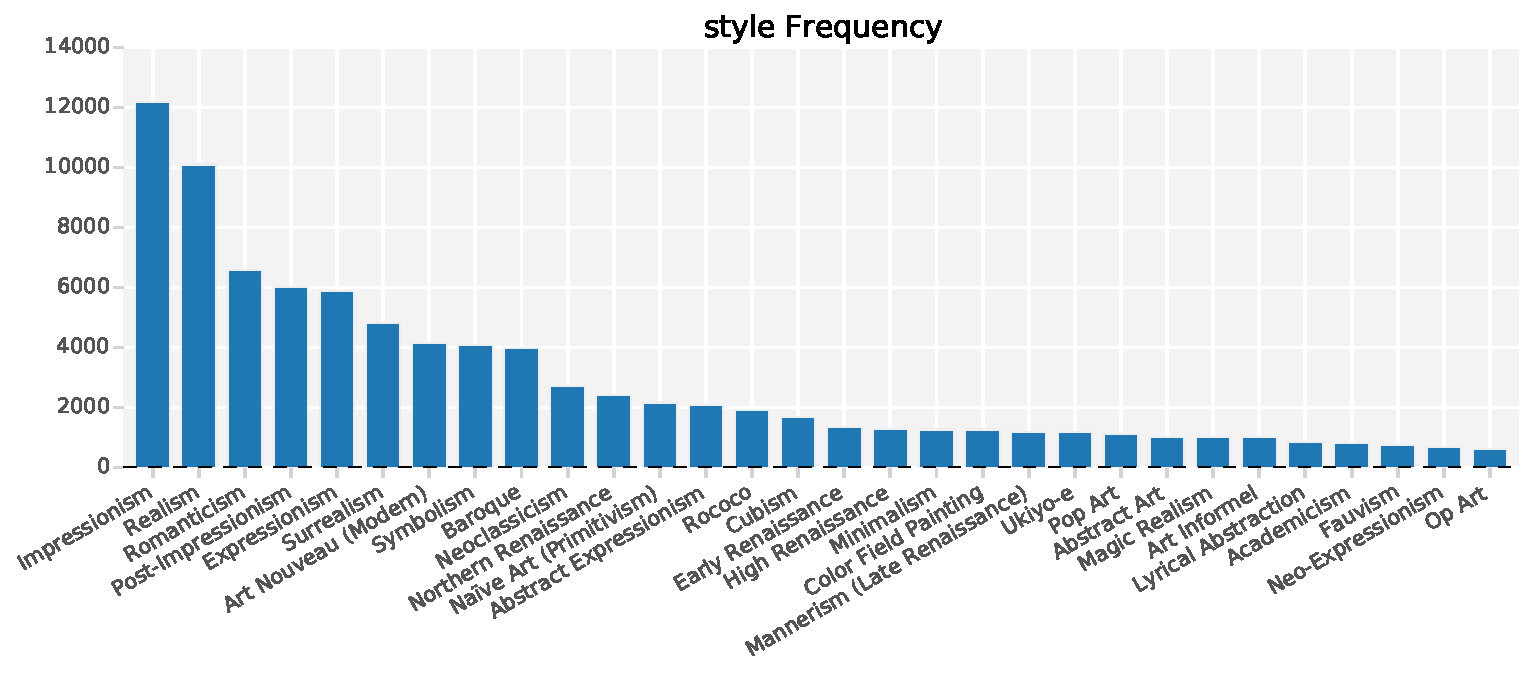
\includegraphics[width=.9\linewidth]{../arxiv/figures/wikipaintings_style.pdf}\\
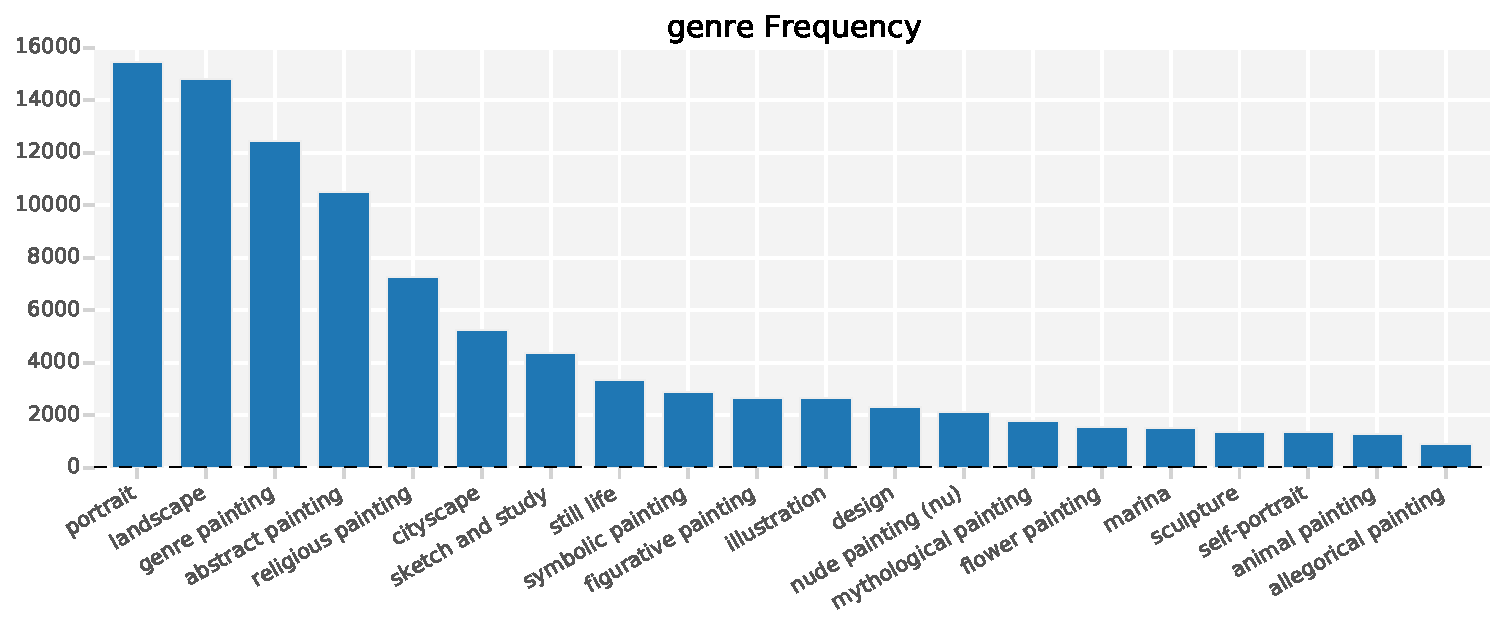
\includegraphics[width=.9\linewidth]{../arxiv/figures/wikipaintings_genre.pdf}\\
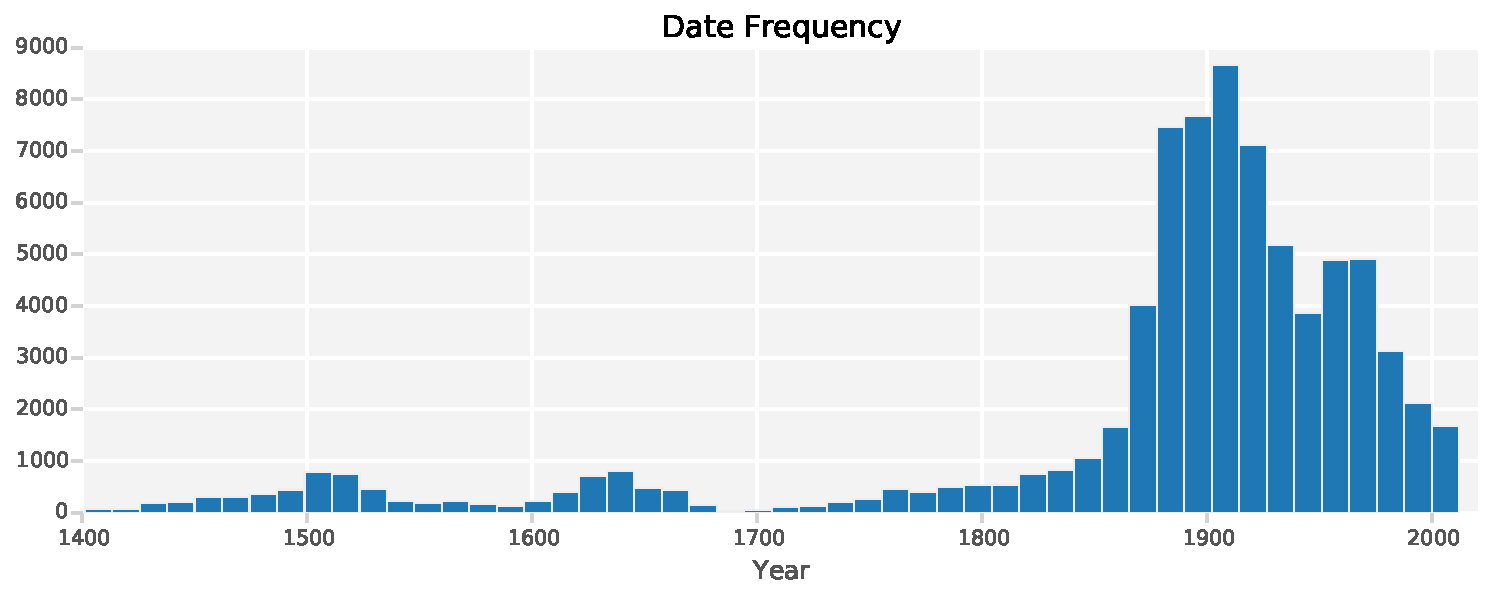
\includegraphics[width=.9\linewidth]{../arxiv/figures/wikipaintings_date.pdf}
\caption{Distribution of image style, genre, and date in the Wikipaintings dataset.}
\label{fig:wikipaintings_data}
\end{figure}
